\documentclass[t,11pt,compress]{beamer} % {{{--
\usefonttheme{serif}
% \documentclass[slidestop,11pt,compress,serif,draft]{beamer} % {{{--

\usepackage{gaelposter}
\usepackage{gaelpython}

% Enlarge margins, this printer is great !
\geometry{verbose, a4paper, left=0.2cm, right=0.2cm, bottom=0pt}

%\usepackage{relsize} % for relative sizes
\usepackage{picins}
\usepackage{graphicx}
\usepackage{multicol}
\usepackage{calc}
\usepackage{agmacros}
\usepackage{color}

% add some MNE + nice colors
\definecolor{mnewebblue}{HTML}{08547D}
\definecolor{mnered}{HTML}{C72219}
\definecolor{mneblue}{HTML}{392FC2}
\definecolor{mnewebgreen}{HTML}{00711B}
\definecolor{mygray}{HTML}{00711B}


\usepackage{pgf}

\graphicspath{{img/}}

%%%%%%%%%%%%%%%%%%%%%%%%%% My box command %%%%%%%%%%%%%%%%%%%%%%%
\usepackage{xkeyval}

\makeatletter
\define@key{mybox}{corners}{\def\my@corners{#1}}
\define@key{mybox}{color}{\def\bg@color{#1}}
\define@key{mybox}{width}{\setlength\mybox@width{#1}}
\define@key{mybox}{position}{\def\box@position{#1}}
\define@key{mybox}{innerposition}{\def\box@innerposition{#1}}
\define@key{mybox}{opacity}{\def\box@opacity{#1}}
\define@key{mybox}{height}{\def\box@height{#1}}
\newbox\my@tempbox
\newlength\my@height
\newlength\my@width
\newlength\mybox@width
\newlength\innerbox@width
\newlength\box@heightlgth

\newcommand{\mybox}[2][]{%
  \setlength\mybox@width{\linewidth}%
  \def\box@position{T}%
  \def\box@innerposition{s}%
  \def\box@opacity{0.75}%
  \def\bg@color{gray!25}%
  \def\my@corners{2mm}%
  \let\box@height\@empty
  \setkeys{mybox}{#1}%
  \setlength\innerbox@width{\mybox@width}%
  \advance\innerbox@width by -2mm%
  \setbox\my@tempbox=\hbox{%
  \ifx\box@height\@empty%
    \begin{minipage}{\innerbox@width}%
  \else%
    \setlength\box@heightlgth{\box@height}%
    \advance\box@heightlgth by -\my@corners%
    \advance\box@heightlgth by -1.7ex%
    \begin{minipage}[\box@position][\box@heightlgth][\box@innerposition]%
        {\innerbox@width}%
  \fi%
      #2%
    \end{minipage}%
  }%
  \my@height=\ht\my@tempbox%
  \my@width=\wd\my@tempbox%
  %
  \advance\my@width by 2mm%
  %
  \begin{minipage}[\box@position]{\mybox@width}%
  \begin{tikzpicture}[rounded corners=\my@corners, fill=\bg@color]
      \fill[fill opacity=\box@opacity, scale=0.5]
          (-\my@width,-2\my@height) rectangle (\my@width, 2\my@height);
      \path (0,0) node {\box\my@tempbox} ;
  \end{tikzpicture}%
  \end{minipage}%
}
\makeatother

%%%%%%%%%%%%%%%%%%%%%%%%%% Poster related style %%%%%%%%%%%%%%%%%
\newcommand{\vfillll}{\vfilll\vfilll\vfilll\vfilll\vfilll\vfilll\vfilll\vfilll\vfilll\vfilll\vfilll\vfilll\vfilll\vfilll\vfilll\vfilll\vfilll\vfilll\vfilll\vfilll\vfilll\vfilll\vfilll\vfilll\vfilll\vfilll\vfilll\vfilll\vfilll\vfilll\vfilll\vfilll\vfilll\vfilll\vfilll\vfilll\vfilll\vfilll\vfilll\vfilll}

\newcommand{\blocktitle}[2]{
    \vfillll%
    \hspace*{-1pt}\mybox[corners=0pt, opacity=1.0, color=#2]{%
    {\sffamily\bfseries\Large%
    \raisebox{-.4ex}{\rule{0pt}{1ex}}%
    \color{white}{#1}}%
    }%
    \vspace*{1.8ex}%
}

\renewcommand{\subsection}[1]{%
\normalsize\emph{\sffamily #1\\[-0.9em]\rule{\linewidth}{1pt}}%
\par%
}

\def\name#1{\mbox{\sc #1}}
\setlength\fboxsep{0pt}

\newcommand{\photoframe}[1]{\setlength\fboxsep{0pt}%
\color{gray}\fbox{#1}}

\newcommand{\mydot}{\hspace*{-0.3ex}%
\raisebox{0.2ex}{\color{mnewebblue}\rule{1.1ex}{1.1ex}}%
\hspace*{0.4ex}%
}

\newcommand{\mydotdot}{\hspace*{1.3ex}%
\raisebox{0.2ex}{\color{alertcolor}\rule{1.1ex}{1.1ex}}%
\hspace*{0.4ex}%
}

\newcommand{\mywhitedot}{\hspace*{0.1ex}%
\raisebox{0.2ex}{\color{white}\rule{1.1ex}{1.1ex}}%
\hspace*{0.4ex}%
}

\newcommand{\green}[1]{{\color{Green!70!black} #1}}
% \newcommand{\green}[1]{{\color{Green!40!black} #1}}

% Def BLOCK environment
\newenvironment{myblock}[1]{
    \blocktitle{#1}{mnewebblue}%
    \vspace*{-1.5ex}%
    \mybox[corners=0pt, color=white, width=\linewidth]{
}{
    }
}

% Def Alert BLOCK environment
\newenvironment{myalertblock}[1]{
    % \blocktitle{#1}{Red!90!black}%
    \blocktitle{#1}{mnered}%
    \vspace*{-1.5ex}%
    \mybox[corners=0pt, color=white, width=\linewidth]{
}{
    }
}

% Def Example BLOCK environment
\newenvironment{myexampleblock}[1]{
    % \blocktitle{#1}{green!40!black}%
    \blocktitle{#1}{mnewebblue}%
    % \blocktitle{#1}{mnewebgreen}%
    \vspace*{-1.5ex}%
    \mybox[corners=0pt, color=white, width=\linewidth]{
}{
    }
}

% Def Filled BLOCK environment
\newenvironment{myfilledblock}[1]{
    \mybox[opacity=1.0, color=alertcolor, width=\linewidth]{%
        \bfseries\sffamily\color{white}
        {\LARGE%
            \raisebox{-.4ex}{\rule{0pt}{0.9em}}%
            #1
        \hrule
        }%
}{
    }
}

% \mybox[opacity=1.0, color=alertcolor, width=.6\linewidth]{%
%     \bfseries\sffamily\color{white}
%     {\LARGE%
%         \raisebox{-.4ex}{\rule{0pt}{0.9em}}%
%         Functional networks
%     \hrule
%     }%
%     Express pathology and cognition
% }

%%%%%%%%%%%%%%%%%%%%%%%%%% Local defines : %%%%%%%%%%%%%%%%%%%%%%
% define a slanted fraction:
% \def\slantfrac#1#2{\kern.1em^{#1}\kern-.3em/\kern-.1em_{#2}}
% define Dirac's braket notation (stolen from braket.sty, that
% unfortunately does not come with TeTeX
% \def\bra#1{\mathinner{\langle{#1}|}}
% \def\ket#1{\mathinner{|{#1}\rangle}}
% \xdefinecolor{darkgreen}{rgb}{0,0.5,0}
% \xdefinecolor{darkred}{rgb}{0.7,0,0}

%%%%%%%%%%%%%%%%%%%%%%%%%%%%%%%%%%%%%%%%%%%%%%%%%%%%%%%%%%%--}}}%
\begin{document}
\newlength\thiscolumnheight

\setbeamertemplate{background}
{%
\rule{0pt}{0.76\paperheight}%
\centerline{%
% \includegraphics[width=.8\linewidth]{pretty_brain_white_transp}%
}%
}%

% \setbeamercolor{normal text}{bg=shadingcolor!25}
% \setbeamercolor{frametitle}{bg=mnewebblue}
\setbeamercolor{normal text}{bg=shadingcolor!25}

\setbeamercolor{frametitle}{bg=mnewebblue, fg=White}
\setbeamercolor{frametitle right}{bg=mnewebblue}
\setbeamercolor{structure}{fg=mnewebblue, bg=mnewebblue}

\beamertemplateshadingbackground{white}{white}
% \beamertemplateshadingbackground{shadingcolor!50}{white}
\begin{frame}[plain,t,c]
\postertitle{%
\smallskip
% Trends in MEG/EEG data processing using MNE
MEG and EEG data processing using MNE:\\
News from the trenches
}
\vspace*{-0.2em}%
%%%%%%%%%%%%%%%%%%%%%%%%%%%%%%%%%%%%%%%%%%%%%%%%%%%%%%%%%%%%%%%%%%%%%%%%%%%%%%%%
% Authors and logos {{{---
% \begin{minipage}{0.165\linewidth}
\begin{minipage}{0.155\linewidth}
    % \vspace{0.5ex}
    \centerline{%
    \hspace{3mm}
    
\includegraphics[width=0.8\linewidth]{logos_left.png}%
    \hspace{3mm}
    }
\end{minipage}
%
\hfill
%
\vspace*{-0.2em}%
\mybox[width=0.67\linewidth, opacity=0., color=white]{%
    \small
    \def\PARISTECH{\unskip$^1$}
    \def\NSPIN{\unskip$^2$}
    \def\UW{\unskip$^3$}
    \def\MGH{\unskip$^4$}
    \def\NYU{\unskip$^5$}
    \def\ILMENAU{\unskip$^6$}
    \def\MARBURG{\unskip$^7$}
    \def\LEUVEN{\unskip$^{8}$}
    \def\UCB{\unskip$^{9}$}
    \def\UCSF{\unskip$^{10}$}
    \def\AALTO{\unskip$^{11}$}

    \begin{center}
    % \vspace*{-0.8ex}%
    \mbox{\hspace{-1em}%
    \name{A. Gramfort\PARISTECH$^{,}$\NSPIN, D.A. Engemann\NSPIN, E. Larson\UW, M. Jas\PARISTECH, C. Brodbeck\NYU}}
    \mbox{\hspace{-1em}%
    \name{T. Brooks\NYU, J. Lepp\"akangas\PARISTECH, M. van Vliet\LEUVEN, C. Brodbeck\NYU, , M. Wronkiewicz\UW}}
    \mbox{\hspace{-1em}
    \name{D. Strohmeier\ILMENAU, J. Sassenhagen\MARBURG, J.R. King\NYU, C. Holdgraph\UCB, Y. Bekhti\PARISTECH}}
    \mbox{\hspace{-1em}
          \name{F. Raimondo\NSPIN, L. Parkkonen\AALTO, M. H\"am\"al\"ainen\MGH$^,$\AALTO}}
	\vspace{0.05cm}
	\def\affilbr{\hspace{0.2cm}}
    \parbox{13cm}{\tiny\center
                 \PARISTECH Telecom ParisTech, CNRS LTCI, Paris, France \affilbr
                 \NSPIN CEA-INSERM Neurospin, Gif-sur-Yvette, France \affilbr\\
                 \UW Univ. of Washington, USA \affilbr
                 \MGH MGH, Harvard Med. School, USA \affilbr
                 \NYU New York Univ., USA \affilbr\\
                 \ILMENAU TU Ilmenau, Germany \affilbr
                 \MARBURG Philipps-Universität Marburg, Germany \affilbr
                 \UCSF UC San Francisco, USA \affilbr
                 \UCB UC Berkeley, USA \affilbr\\
                \AALTO Aalto Univ., Espoo, Finland \affilbr
                 }
    \end{center}
}
%
\hfill
%
\begin{minipage}{0.15\linewidth}
    \vspace{0ex}
    \hfill
    \centerline{%
    
\includegraphics[width=0.188\linewidth]{logo_telecom}
    \,
    
\includegraphics[width=0.233\linewidth]{logo_cea}
    \,
    
\includegraphics[width=0.45\linewidth]{logo_tuil}
    }
    \centerline{%
    
\includegraphics[width=0.24\linewidth]{logo_uw}
    \,
    
\includegraphics[width=0.45\linewidth]{logo_fzj_cut}
    \,
    
\includegraphics[width=0.21\linewidth]{logo_cns}
    }
    \centerline{%
    
\includegraphics[width=0.25\linewidth]{logo_icm.png}
    \,
    
\includegraphics[width=0.4\linewidth]{logo_bu.png}
    }

\end{minipage}

%\begin{minipage}{0.14\linewidth}
%    \hfill
%    \centerline{%
%    
\includegraphics[width=0.25\linewidth]{logo_telecom}
%    \,
%    
\includegraphics[width=0.31\linewidth]{logo_cea}
%    \,
%    
\includegraphics[width=0.35\linewidth]{logo_uw}
%    }
%    \centerline{%
%    \,
%    
\includegraphics[width=0.60\linewidth]{logo_fzj}
%    \,
%    
\includegraphics[width=0.30\linewidth]{logo_cns}
%    }
%
%\end{minipage}

%%%%%%%%%%%%%%%%%%%%%%%%%%%%%%%%%%%%%%%%%%%%%%%%%%%%%%%%%%%%%%%%%%%%%%%%%%%%%%%%
% ---}}}

\sffamily
\vfillll%

% First row {{{---
%%%%%%%%%%%%%%%%%%%%%%%%%%%%%%%%%%%%%%%%%%%%%%%%%%%%%%%%%%%%%%%%%%%%%%%%%%%%%%%%
%-------------------------------------------------------------------------------

% \smallskip

\vspace*{-0.5em}%  
\begin{minipage}[B]{0.47\linewidth}
    \vspace*{-0.5em}%
    \begin{myalertblock}{The MNE Software Vision}
        \mydot State-of-the-art methods, documented and tested\\
        \mydot Open development: collaboration between several centers\\
        \mydot Share the best practices, promote reproducible research\\
    \end{myalertblock}
    % \smallskip
    \vspace*{-0.6em}%
    \begin{myexampleblock}{Software Features}
        \subsection{Preprocessing}
        \mydot Review raw data, filter, artifact reduction with SSP, ICA\\
        \subsection{Forward \& inverse modeling}
        \mydot Forward modeling with FreeSurfer-generated surfaces\\
        \mydot MNE -- dSPM -- sLORETA -- (TF-)MxNE -- LCMV -- DICS\\
        %\mydot Dipole fitting -- RAP-MUSIC\\
        \subsection{Statistics (sensor and source spaces)}
        \mydot Time--Frequency (Phase-Locking, Induced Power)\\
        \mydot Parametric and non-parametric stats, with clustering\\
        \mydot Decoding/MVPA (SVM, ...), CSP, Time decoding\\
        \subsection{Connectivity (sensor and source spaces)}
        \mydot Functional and effective connectivity measures
    \end{myexampleblock}

\end{minipage}%
%
\hfill%
\begin{minipage}{.52\linewidth}
    \vspace{0.5em}
    \begin{minipage}{\linewidth}
    \subsection{What's new}
    \mydot Maxwell Filter (SSS), dipole fitting, RAP-MUSIC, interpolation of bad EEG/MEG channel, automated covariance regularization, multi-taper time-frequency, deep structures in source spaces, basic ECoG support, segment annotations,
    interactive viz (TFR \& ERP)\\
    \mydot \url{http://martinos.org/mne/dev/whats\_new.html}
    \begin{center}
        \vspace*{-1.em}%
        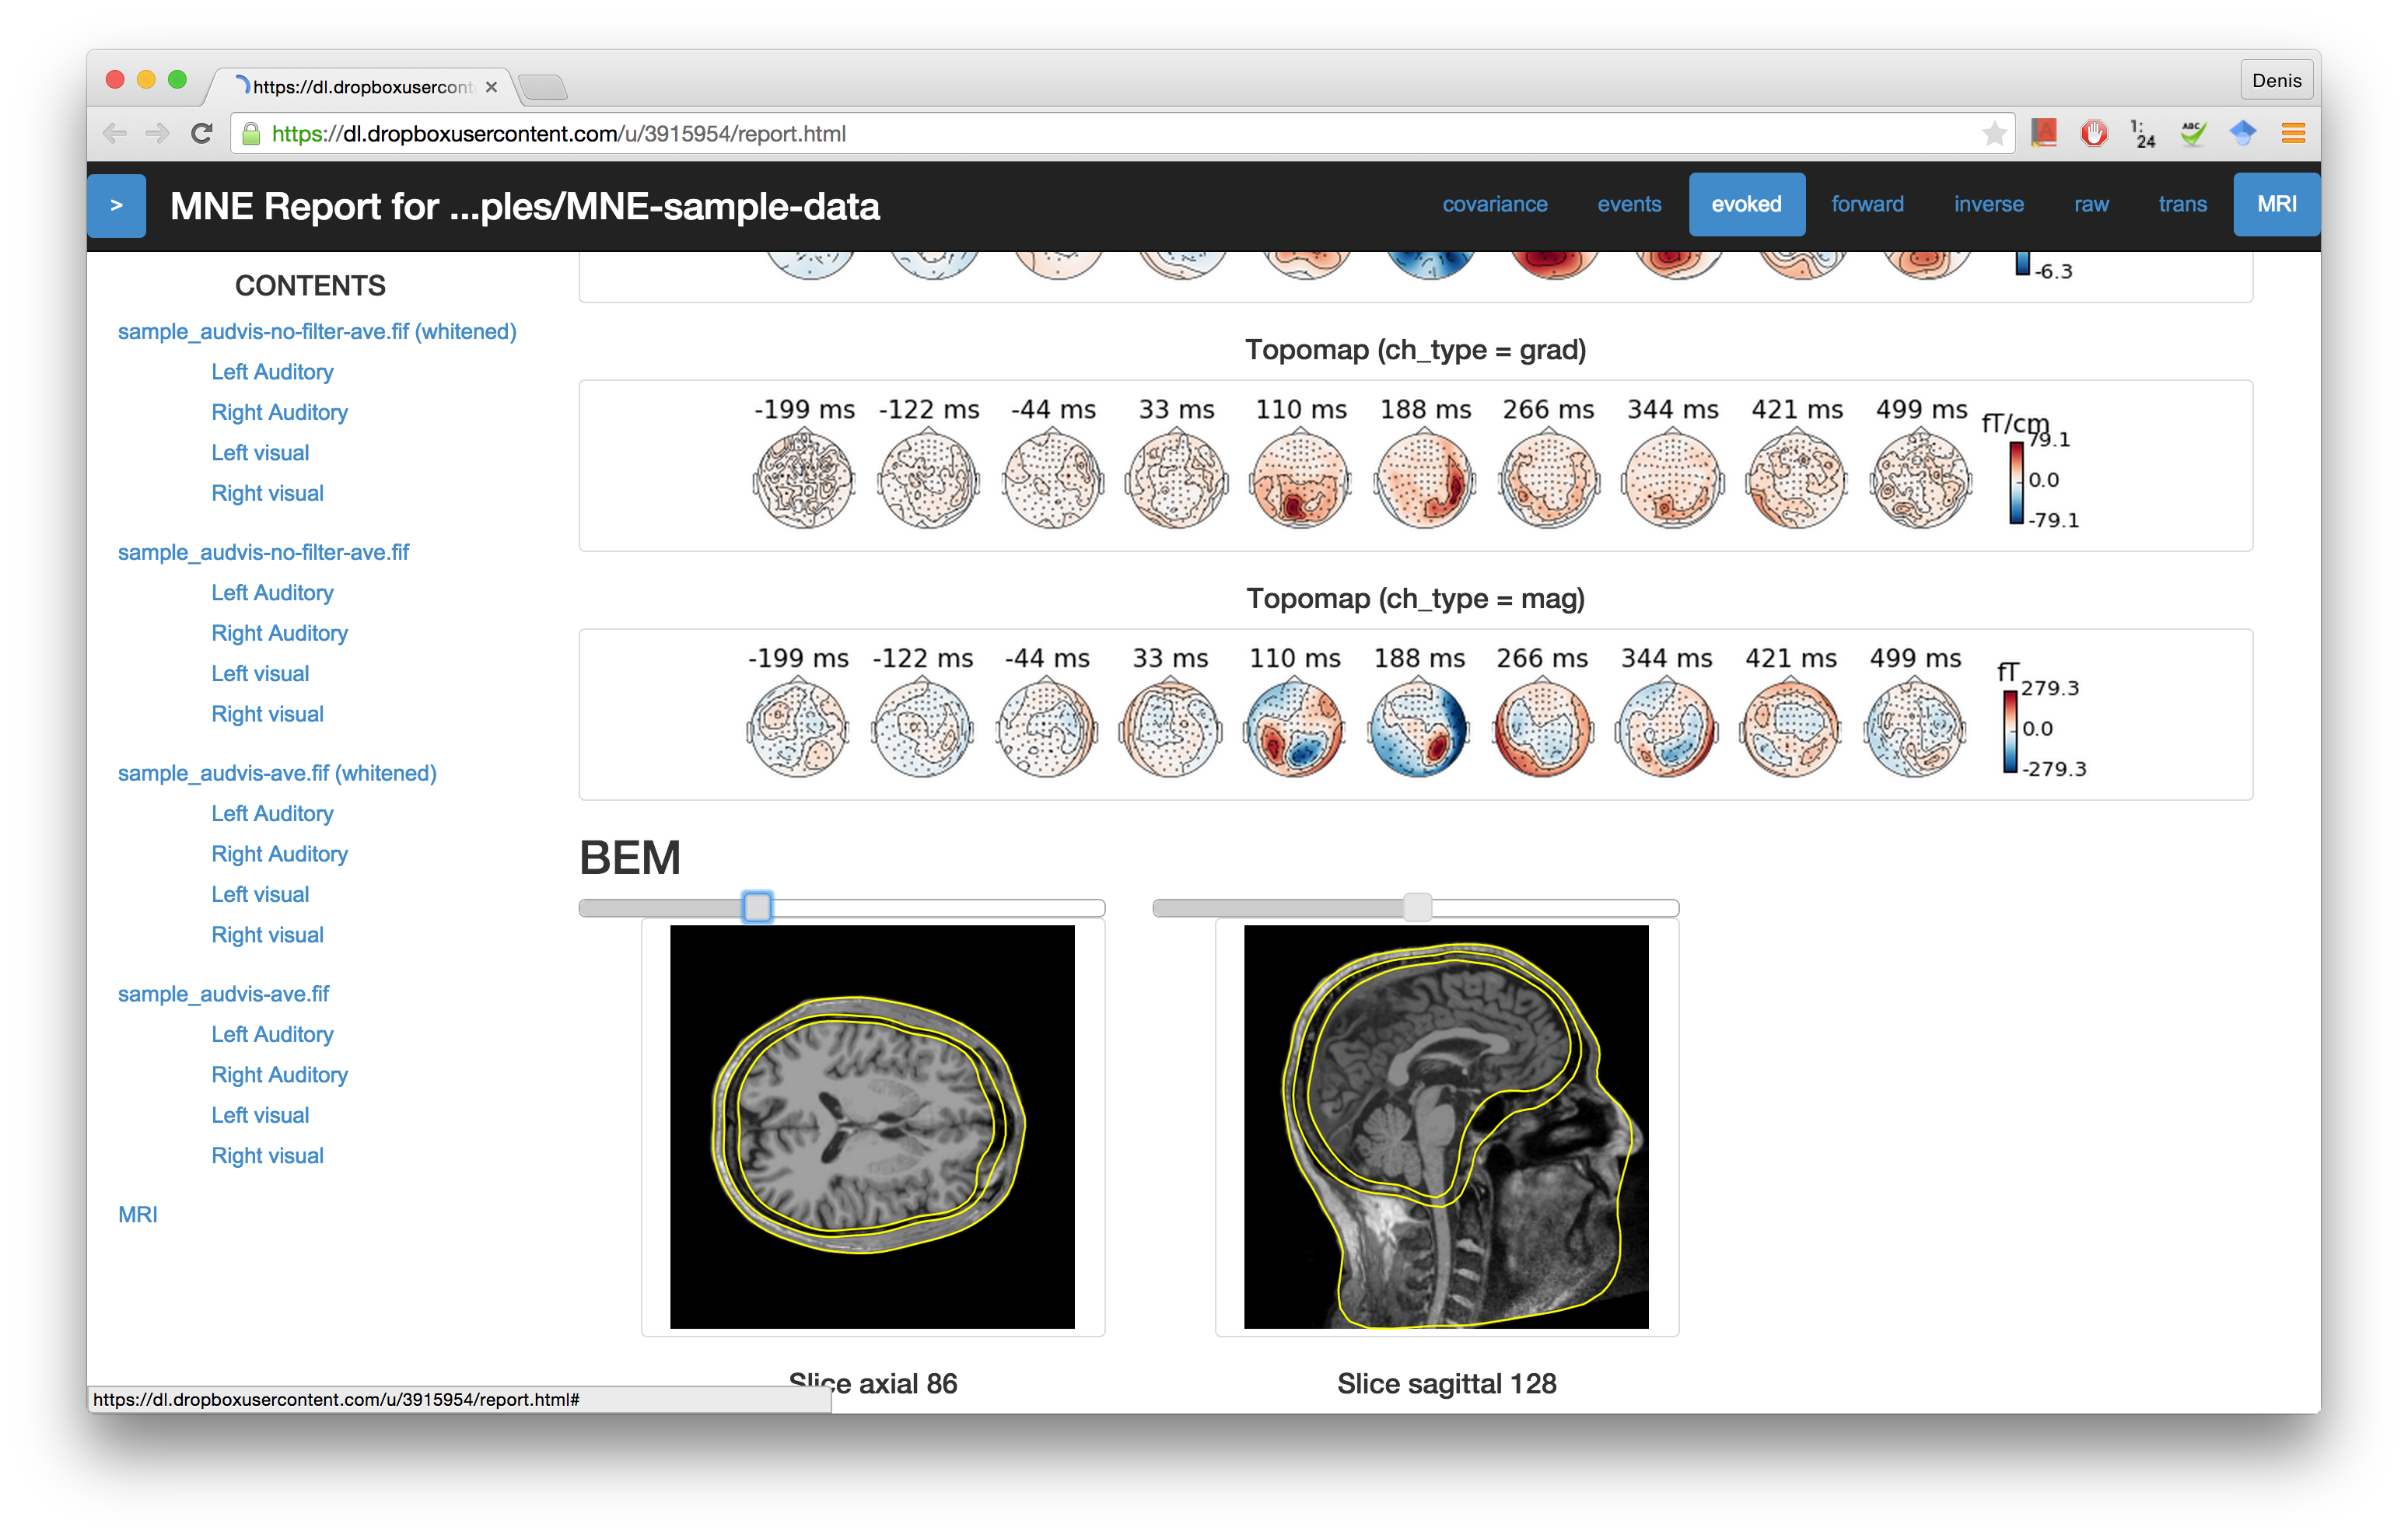
\includegraphics[width=0.95\linewidth]{mne_report.png}%
    \end{center}
    \end{minipage}
\end{minipage}
% First row ---}}}

\begin{minipage}{\linewidth}
    \smallskip
    \vspace*{-0.3ex}%
\center
{\huge\bfseries\sffamily http://martinos.org/mne~~~~~~http://github.com/mne-tools}
\end{minipage}

\begin{minipage}{\linewidth}
\smallskip
\centering
\begin{minipage}{0.05\linewidth}
    
\includegraphics[width=0.9\linewidth]{paper_logo.pdf}%
\end{minipage}
\begin{minipage}{0.93\linewidth}
    A. Gramfort, M. Luessi, E. Larson, D. Engemann, D. Strohmeier, C. Brodbeck, L. Parkkonen, M. H\"am\"al\"ainen\hfill\\
    \emph{MNE software for processing MEG and EEG data}, Neuroimage, 2014
\end{minipage}\\
\begin{minipage}{0.05\linewidth}
    
\includegraphics[width=0.9\linewidth]{paper_logo.pdf}%
\end{minipage}
\begin{minipage}{0.93\linewidth}
    A. Gramfort, M. Luessi, E. Larson, D. Engemann, D. Strohmeier, C. Brodbeck, R. Goj, M. Jas, T. Brooks, L. Parkkonen, M. H\"am\"al\"ainen,
    \emph{MEG and EEG data analysis with MNE-Python}, Frontiers in Neuroscience, 2013
\end{minipage}
\end{minipage}
% \medskip
% \vfillll

% Bottom banner {{{---
%%%%%%%%%%%%%%%%%%%%%%%%%%%%%%%%%%%%%%%%%%%%%%%%%%%%%%%%%%%%%%%%%%%%%%%%%%%%%%%%

% \begin{minipage}{.4\linewidth}
%     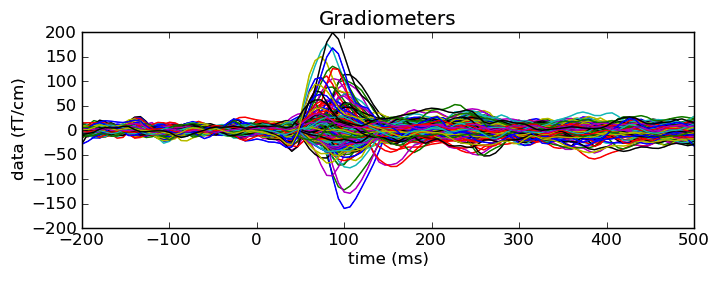
\includegraphics[width=\linewidth]{plot_evoked.png}%
% \end{minipage}%
% \hfill%
% \begin{minipage}{.4\linewidth}
%     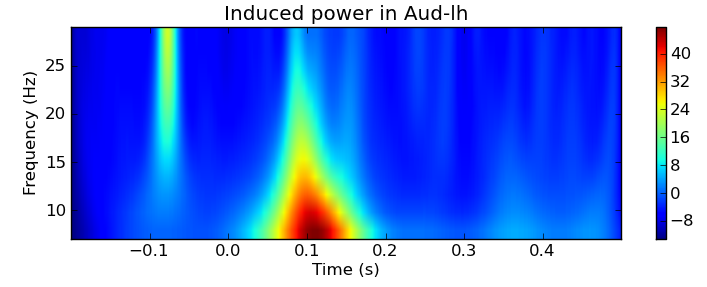
\includegraphics[width=\linewidth]{induced.png}%
% \end{minipage}%
% \hfill%
% \begin{minipage}{.18\linewidth}
%     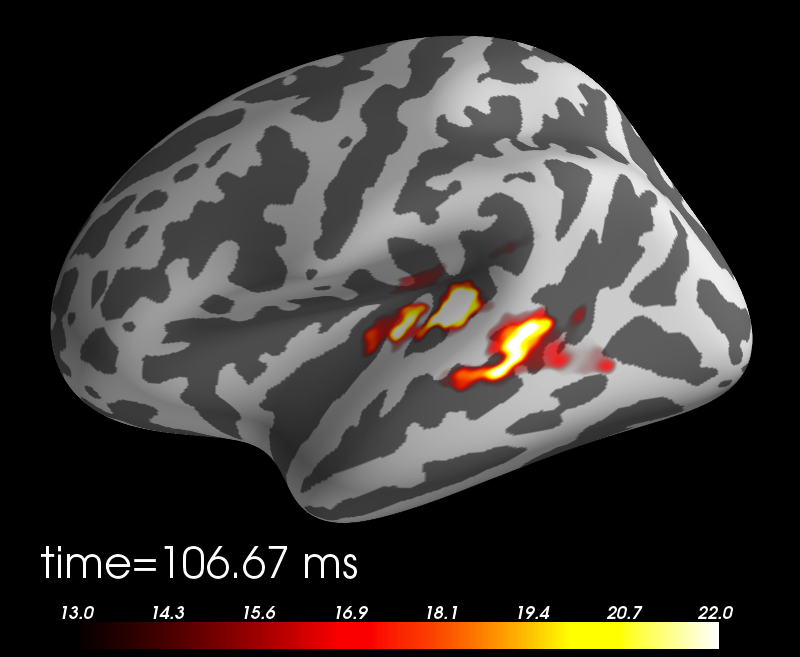
\includegraphics[width=\linewidth]{pysurfer.png}%
% \end{minipage}%
% \hfill%
% % \begin{minipage}{.19\linewidth}
% %     \includegraphics[width=\linewidth]{nonlinear_svm}
% %     \llap{\raisebox{15ex}{Custom kernel SVM ~}}
% % \end{minipage}%
% \hfill%
% Second row ---}}}

% Second row {{{---
%%%%%%%%%%%%%%%%%%%%%%%%%%%%%%%%%%%%%%%%%%%%%%%%%%%%%%%%%%%%%%%%%%%%%%%%%%%%%%%%

\begin{minipage}{\linewidth}
    \begin{minipage}[t]{0.48\linewidth}
        \begin{myexampleblock}{MNE-Python}
            \mydot Python: general-purpose, high-level language \\
            \mydot Free: can run on a cluster without license problems\\
            \mydot Permissive BSD license: allows use in commercial products\\
            \mydot 47 contributors in last 12 months $\approx$ 13 person-years of effort
            \begin{center}
                \vspace{-0.5em}
                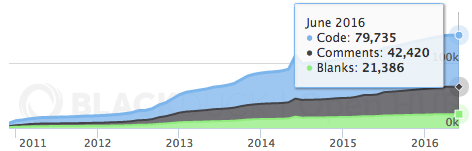
\includegraphics[width=0.9\linewidth]{sloc_june_2016_v2.png}%
            \end{center}
        \end{myexampleblock}
        \vspace{-0.8em}
        \begin{myalertblock}{Learn more}
            \begin{minipage}{1.\linewidth}
                \mydot Mailing list: mne\_analysis@nmr.mgh.harvard.edu\\
                \mydot http://martinos.org/mne/ (general doc)\\
                \mydot http://martinos.org/mne/stable/getting\_started.html\\
                \mydot http://martinos.org/mne/stable/tutorials.html\\
                \mydot http://martinos.org/mne/auto\_examples/ (>90 demos)\\
            \end{minipage}
        \end{myalertblock}
    \end{minipage}
    \begin{minipage}[t]{0.5\linewidth}
        \begin{myexampleblock}{From raw to dSPM in < 30 lines of code}
        \hspace*{.01\linewidth}%
        \vspace{-0.3cm}
        \inputpython{short_example.py}
        \end{myexampleblock}
    \end{minipage}
    \hfill
\end{minipage}

\vfillll

% Second row ---}}}

\vfillll

\vspace*{-2.2em}%

% Bottom banner {{{---
%%%%%%%%%%%%%%%%%%%%%%%%%%%%%%%%%%%%%%%%%%%%%%%%%%%%%%%%%%%%%%%%%%%%%%%%%%%%%%%%

\begin{minipage}{1.09\linewidth}

\hspace{-0.1em}%
\begin{minipage}{.25\linewidth}
    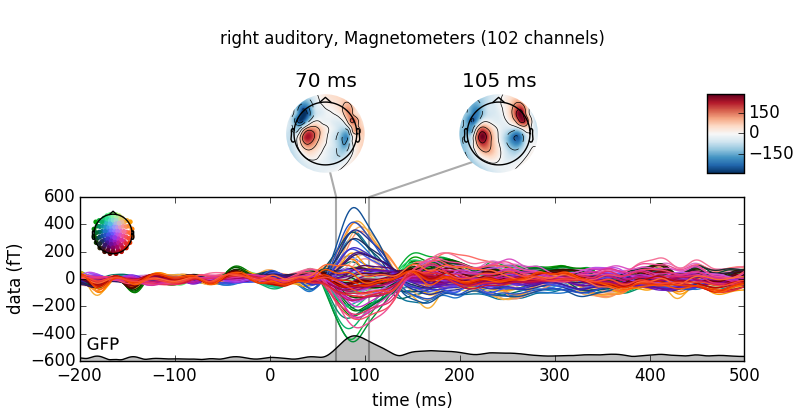
\includegraphics[width=\linewidth]{img/joint_plot.png}
    %dspm_volumetric_cropped.png
\end{minipage}%
\begin{minipage}{.225\linewidth}
    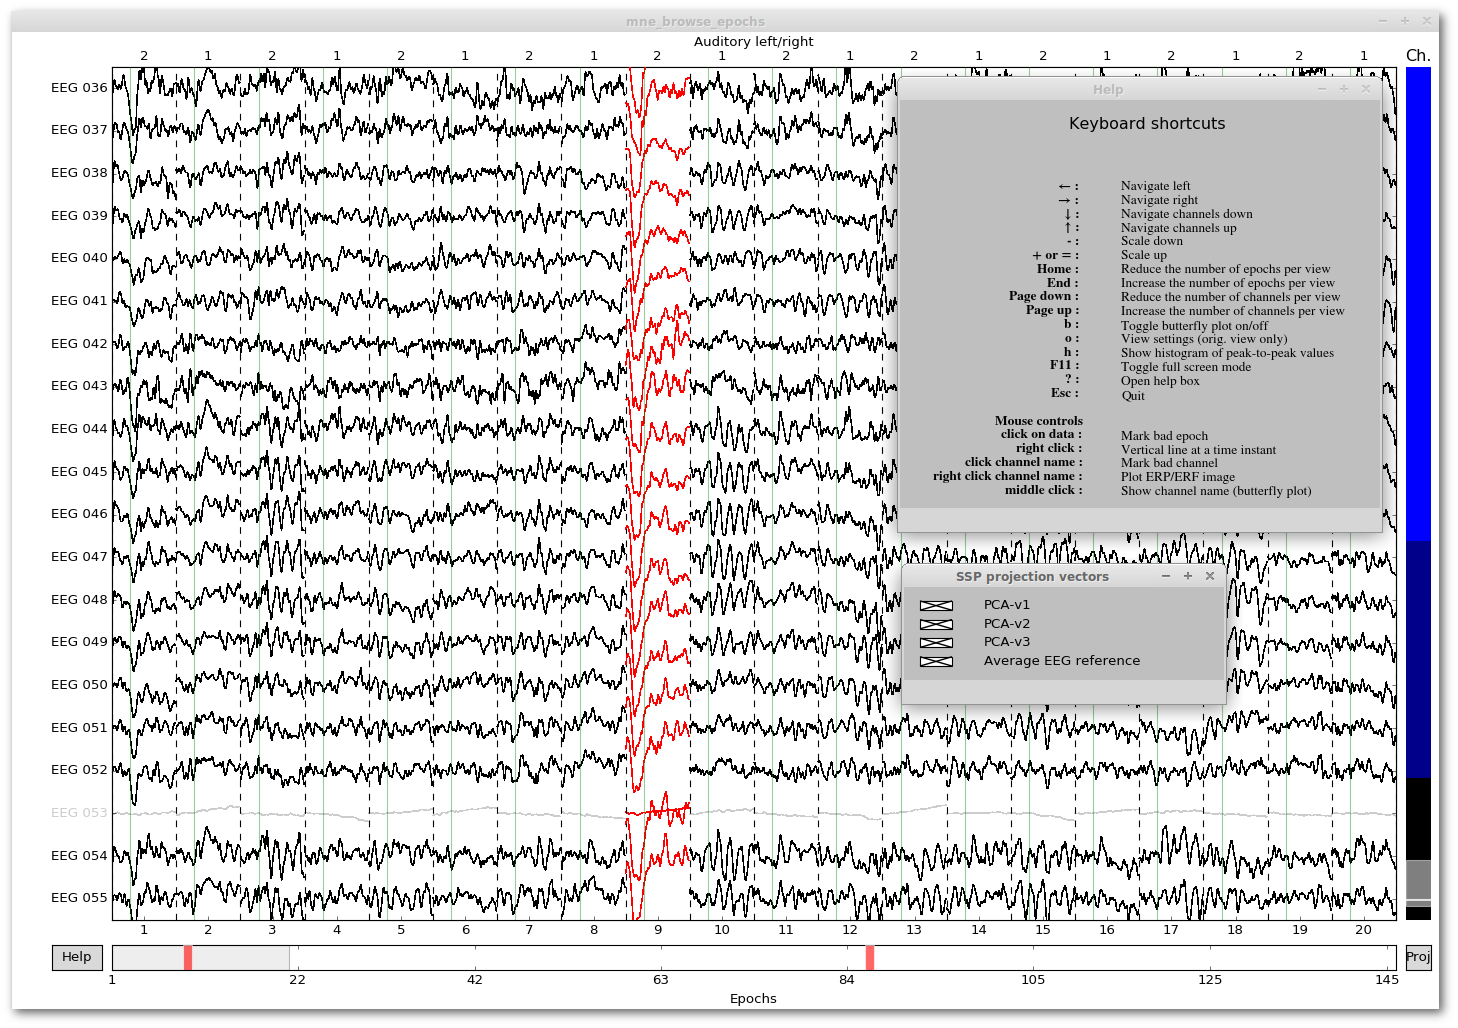
\includegraphics[width=0.85\linewidth]{img/epochs_plotter.png}%
\end{minipage}%
\hspace{-2.0em}%
\hspace{-.4em}%
%\begin{minipage}{.165\linewidth}
%    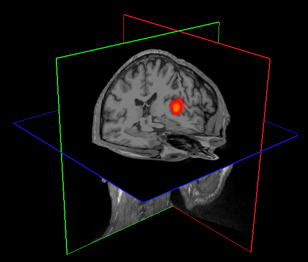
\includegraphics[width=\linewidth]{volume_tc.png}%
%\end{minipage}%
\hspace{.4em}%
\begin{minipage}{.305\linewidth}
    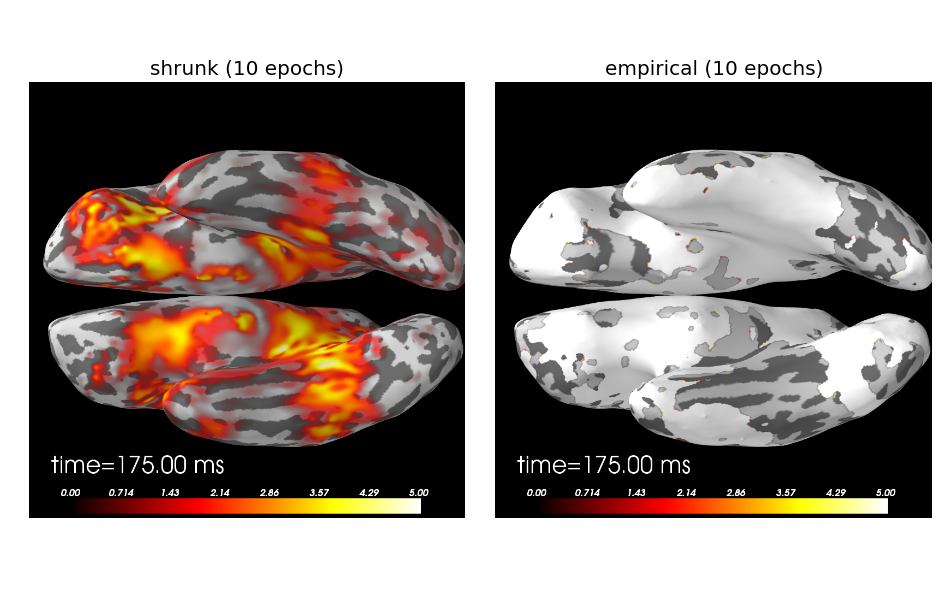
\includegraphics[width=\linewidth]{covariance_whitening_hbm.png}%
\end{minipage}
\hspace{-1.0em}%
\begin{minipage}{.22\linewidth}
    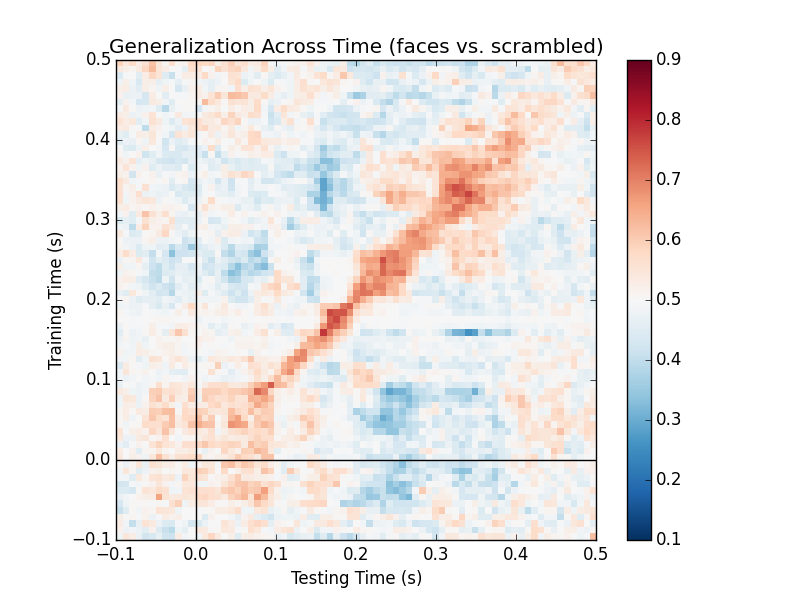
\includegraphics[width=\linewidth]{time_gen.png}%
\end{minipage}
% \medskip
\vspace{1em}%
\end{minipage}
% \begin{minipage}{\linewidth}
%     \vspace*{-0.5em}%
%     \center
%     Funded by: NIH grants P41RR14075, R01EB009048, F32DC012456 and NSF awards 0958669, 1042134
% \end{minipage}
\smallskip
~
\end{frame}
\end{document}
